\documentclass[a4paper,titlepage,10pt]{article}

\usepackage[margin=0.7in]{geometry} % margenes
\usepackage[spanish]{babel} % Le indicamos a LaTeX que vamos a escribir en español.
\usepackage[utf8]{inputenc} % Quiero acentos
\usepackage{caratula}
\usepackage{verbatim} % Para hacer código
\usepackage{graphicx} % Graficos
\usepackage[space]{grffile} % Espacios en el nombre de archivo de includeGraphics


\titulo{Super Collider}
\fecha{23 / 10 / 2013}
\materia{Teoría de Lenguajes}
\grupo{Grupo 4}
\integrante{Carreiro, Martin}{45/10}{martin301290@gmail.com}
\integrante{Kujawski, Kevin}{459/10}{kevinkuja@gmail.com}
\integrante{Ortiz De Zarate, Juan Manuel}{403/10}{jmanuoz@gmail.com}

\begin{document} % Todo lo que escribamos a partir de aca va a aparecer en el documento.

\maketitle

\section{Gramática}

\begin{verbatim}
S -> G | S.P | SOS | {S}
O -> ; | con | & | mix | + | add | - | sub | * | mul | / | div
G -> sin(N,R) | lin(R,R) | linear(R,R) | silQ | silenceQ | noise(R) | noi(R) | R | noise | sin(N)
P -> play(R) | postQ | loop(N) | tune (E) | fill(R) | reduceQ | expandQ | playQ
N -> 0|..|9|0N|1N|..|9N
M -> ZN.N
R -> N | M | E
E -> +N | -N 
Z -> + | - | lambda
Q -> () | lambda

\end{verbatim}

Descripcion:
Basicamente la gramatica se puede dividir en tres categorias cuyo resultando siempre seran buffers: Generadores, Metodos (con parentesis opcionales si no tienen parametros) y Numeros, que estos ultimos a su vez se dividen en enteros, naturales y racionales, para que cada metodo reciba el tipo de parametro que le corresponde. Además, adaptamos la gramatica para que permita los ejemplos del enunciado que no cumplen las formas de escritura por considerarlos como abrevaciones o parametros opcionales de los mismos. 
La presencia de "espacios" no son considerados y son eliminados por el analizador lexico.

Tokens Lexicos:
con
mix
add
sub
mul
div
sin(
lin(
linear(
noi
noise
sil
silence
play(
post
loop(
tune(
fill(
reduce
expand
play
()

\section{Árboles De Derivación}

\centerline{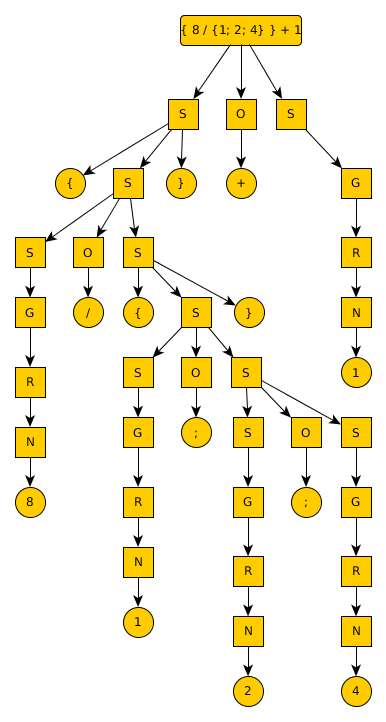
\includegraphics[scale=0.5]{arbolDerivacion2.png}}   

\centerline{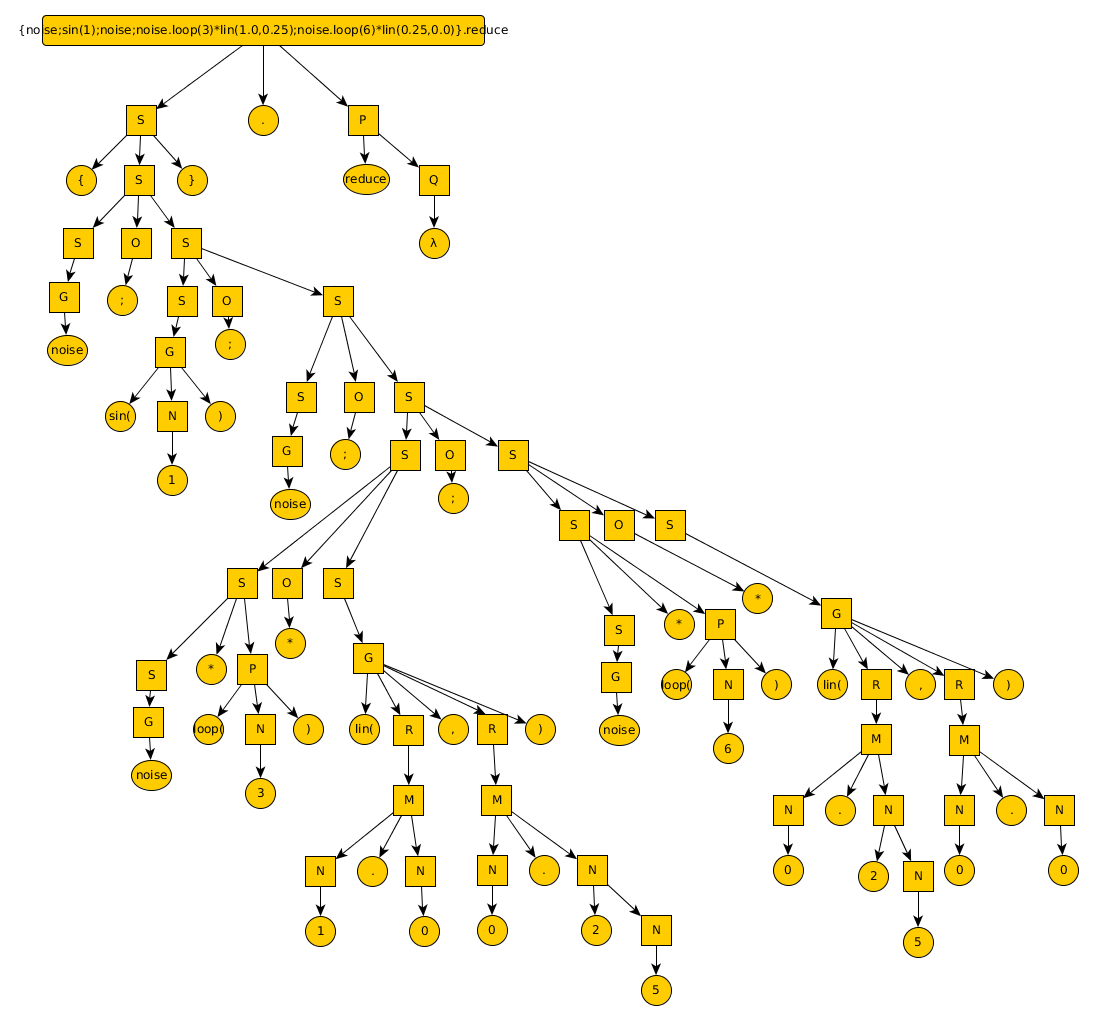
\includegraphics[scale=0.5]{arbolDerivacion.png}}   


\end{document} %Terminé!
